\RequirePackage{plautopatch}
\documentclass[report,a4paper,uplatex,dvipdfmx,11pt]{jsbook}
\usepackage{amsmath,amssymb}
\usepackage{amsfonts}
\usepackage{bm} %数式中でボールド体も斜体にする。\bm{a}と書けば、斜体ボールドのaが書ける
\usepackage{graphicx}
\usepackage[sort,compress,numbers]{natbib} % apsrev4-2ja.bstを使うのに必要
\usepackage{doi}
\usepackage{hyperref}
\bibliographystyle{apsrev4-2ja} % アメリカ物理学会(APS)の標準のbibtexスタイルファイルの適用
%\bibliographystyle{junsrt} % 文献のタイトルまで表示したい場合はこちらを使う


% 余白の設定をするためのパッケージ------------------------------
%\usepackage[pass]{geometry}
%\usepackage{bxpapersize}
% --------------------------------------------------------------


% 章見出しの上の余白を小さくする--------------------------------
\usepackage{etoolbox}
\makeatletter
\patchcmd{\@makechapterhead}{\vspace*{2\Cvs}}{}{}{}
\patchcmd{\@makeschapterhead}{\vspace*{2\Cvs}}{}{}{}
\makeatother
% --------------------------------------------------------------


% 目次のフォントについて----------------------------------------------------
% 1. 見出しの文字を明朝体にする(太字にはならない)
%\renewcommand{\headfont}{\mcfamily}

% 2. 明朝体の太字を使う場合は、上のはコメントアウトして、次の2行を用いる
%\usepackage[deluxe]{otf}
%\renewcommand{\headfont}{\mcfamily\bfseries}

% 3. 見出し全てではなく、目次のフォントのみ変更する場合は、
\usepackage{tocloft}
\renewcommand{\cftchapnumwidth}{3.8em}
\renewcommand{\cftchapfont}{\mcfamily}
\renewcommand{\cftchappagefont}{\rmfamily}
% --------------------------------------------------------------------------


\setcounter{tocdepth}{2} % 目次にどのレベルのセクションまで反映させるか。2だとsubsectionまで。

%\allowdisplaybreaks % 数式の途中での改ページを許す


% 卒論で、図をページ数に含めたくないときに用いる図・表環境-------------
\newenvironment{clearpagefigure}
{
\clearpage
\begin{figure}
\centering
\thispagestyle{empty}
\addtocounter{page}{-1}
}
{\end{figure}}
\newenvironment{clearpagetable}
{
\clearpage
\begin{table}
\centering
\thispagestyle{empty}
\addtocounter{page}{-1}
}
{\end{table}}
% ---------------------------------------------------------------------



\title{卒論・修論用LaTeXテンプレート}
\author{Author's Name}
%\date{2022/01/17}
\date{最終更新: \today}

\begin{document}

\maketitle

\frontmatter
\chapter*{摘要}
\label{chap:abstract}

\tableofcontents

\mainmatter
\chapter{基本的な使い方}
%\label{chap:chapter1}
chapter, section, subsectionや図の挿入、文献引用などのやり方は、本章のソースファイル(chapter1.tex, reference.bib)と出力されたpdfファイルを見比べればわかる。
\section{文献引用の仕方}
このテンプレートでは、BibTeXを使えるようにしている。

また、文献リストのフォーマットは、\url{https://yosuke-nakata.net/2020/04/15/923}からダウンロードした``apsrev4-2ja.bst''というbibtexスタイルファイルを使用している。
これは、アメリカ物理学会(APS)の標準のbibtexスタイルファイル"apsrev4-2.bst"を改造して、日本語の本も表示できるようにしたものらしい。
他にも、APA-likeなスタイルも選べるようにしている。
\subsection{BibTeXの使い方}
文献の引用は、例えば\cite{Okuda2013a}のように行う(ソースファイルchapter1.tex参照)。 
%番号ではなく,著者名・年で引用したい場合は,main.texで\usepackage[sort,compress]{natbib}を使い(numbersを消す),\citepにする
%その場合は,apsrev4-2ではなくapalikeを使う
reference.bibのファイルに文献リストを登録しておけば、
このようにするだけで、自動的に文献リストが作成される。
書籍の場合はarticleではなくbookにする(引用例:\cite{jt})。

reference.bibファイルに入力する内容は、Google Scholarなどから引っ張ってくる。
Google Scholarで引用のマーク(図\ref{fig:googleScholar})をクリックすると、
図\ref{fig:quote}のようなものが出てくる。
\footnote{図の挿入・参照方法はchapter1.texのこの文章の箇所および末尾に並んでいるfigure環境を参照。}
次に、BibTeXをクリックすると、図\ref{fig:bibtex}のようなテキストが出てくる。
\footnote{卒論で図のページをカウントしないようにするためのclearpagefigure環境(main.texで定義)の使い方は、chapter1.texのこの図\ref{fig:bibtex}の挿入をしている箇所を参照。}
これをreference.bibにコピペする(ただし、Google Scholarのcitationはたまにおかしいのが出てくるので、信用し過ぎない方がいい。論文誌のウェブページからもbibtex用のcitationの情報はダウンロードできることがあり、その方が信用できる)。

\begin{figure}[htbp]
	\centering
	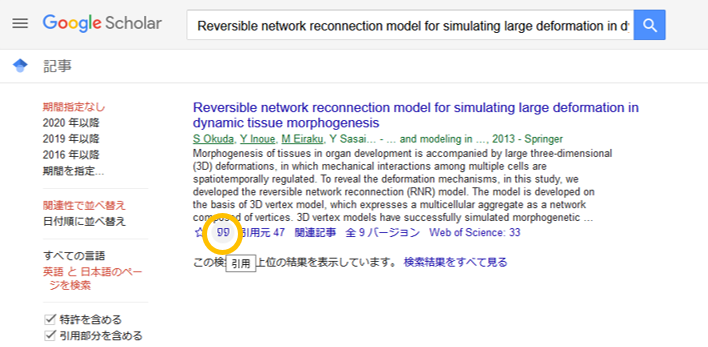
\includegraphics[width=12cm,clip]{fig/googleScholar.png}
	\caption{Google Scholarでの検索結果。引用のマークをクリックする。}
	\label{fig:googleScholar}
\end{figure}

\begin{figure}[htbp]
	\centering
	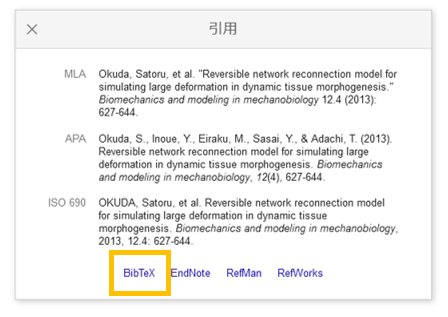
\includegraphics[width=10cm,clip]{fig/quote.png}
	\caption{引用のポップアップ。BibTeXをクリックする。}
	\label{fig:quote}
\end{figure}

% main.texで定義したclearpagefigure環境を使う場合は、
\begin{clearpagefigure}%[htbp]
	%\centering
	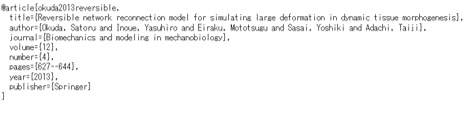
\includegraphics[width=12cm,clip]{fig/bibtex.png}
	\caption{BibTeX. これを.bibファイルにコピペする。}
	\label{fig:bibtex}
\end{clearpagefigure}

\chapter{タイトル}
%\label{chap:chapter2}

\chapter{タイトル}
%\label{chap:chapter2}

\chapter{タイトル}
%\label{chap:chapter4}

\chapter{タイトル}
%\label{chap:chapter5}


\newcounter{pagenumberbody}
\setcounter{pagenumberbody}{\value{page}}

\appendix
\setcounter{page}{1}
\renewcommand{\thepage}{A--\arabic{page}}
\chapter*{付録A}
%\label{chap:appendixA}

\setcounter{page}{1}
\renewcommand{\thepage}{B--\arabic{page}}
\chapter{タイトル}
%\label{chap:appendixB}


\renewcommand{\thepage}{\arabic{page}}
\setcounter{page}{\value{pagenumberbody}}

\backmatter
\bibliography{reference} % reference.bibの読み込み

\chapter*{謝辞}
%\label{chap:acknowledgement}



\end{document}
